\documentclass[a4paper]{article}

\usepackage[utf8]{inputenc}
\usepackage[T1]{fontenc,url}
\usepackage{cite}
\usepackage{hyperref}
\usepackage{amsmath, amssymb}
\usepackage{tikz}
\usepackage{graphicx}
%\usepackage{subcaption}
\usepackage{parskip}
\usepackage{lmodern}
\usepackage{algorithm}
\usepackage{algpseudocode}
\usepackage{epigraph}
\usepackage{listings}
\usepackage{physics}
\usepackage{varioref}

% varioref stuff from Anders
\labelformat{section}{section~#1}
\labelformat{subsection}{section~#1}
\labelformat{subsubsection}{paragraph~#1}
\labelformat{equation}{(#1)}
\labelformat{figure}{figure~#1}
\labelformat{table}{table~#1}



\begin{document}
\title{FYS3150 -- Project 3}
\author{
    \begin{tabular}{r l}
        Kristian Gregorius Hustad & (\texttt{krihus})\\
        Jonas Gahr Sturtzel Lunde & (\texttt{jonassl})
    \end{tabular}}
%\date{}    % if commented out, the date is set to the current date

\maketitle




% quote
\setlength{\epigraphwidth}{0.75\textwidth}
\renewcommand{\epigraphflush}{center}
\renewcommand{\beforeepigraphskip}{50pt}
\renewcommand{\afterepigraphskip}{100pt}
\renewcommand{\epigraphsize}{\normalsize}

\epigraph{Rockets are cool. There's no getting around that.}
{\textit{Elon Musk}}

% alternative quote
%\epigraph{The first principle is that you must not fool yourself -- and you are the easiest person to fool.}{\textit{Richard Feynman}}

\begin{abstract}
\noindent
In this report, ...

\textbf{Fill in abstract}
\end{abstract}

\vfill


\begin{center}
    GitHub repository at \url{https://github.com/KGHustad/FYS3150}
\end{center}

\newpage

%%% MACROS
\newcommand{\half}{\frac{1}{2}}
\newcommand{\dt}{{\Delta t}}
\newcommand{\dx}{{\Delta x}}
\newcommand{\bigO}{{\mathcal{O}}}

\newcommand{\supnew}{^{\mathrm{new}}}



\section{Introduction}\label{sec:intro}
%\subsection*{Description of the nature of the problem}
\cite{mhj_lecture_notes} % must cite something to avoid compilation error when using bibtex

In this report, we aim to study the solar system and the motion of celestial bodies in a gravitational field.



\textbf{Fill in introduction}



\section{Discussion of methods}\label{sec:methods}
Newton's law of universal gravitation dictate that, for two celestial bodies, $\alpha$ and $\beta$, the force of attraction between the two is given by
\begin{equation}
F_G
=\frac{Gm_{\beta}m_{\alpha}}{r_{\alpha \leftrightarrow \beta}^2}
\label{eq:grav:newton}
\end{equation}

%For circular orbits, we additionally have
%\begin{equation}
%    F_G= \frac{m_{\alpha}v_{\alpha}^2}{r_{\alpha \leftrightarrow \beta}}
%\end{equation}

Here $v_{\alpha}$ is the velocity of $\alpha$ relative to the system's center of mass, which we will keep in origo, and $r_{\alpha \leftrightarrow \beta}$ is the distance between $\alpha$ and $\beta$
\begin{equation}
r_{\alpha \leftrightarrow \beta} = \norm{ \vec{x}_{\alpha} - \vec{x}_{\beta} }
\end{equation}

\ref{eq:grav:newton} can be adjusted to account for Einstein's theory of relativity, yielding
\begin{equation}
F_G
=\frac{Gm_{\beta}m_{\alpha}}{r_{\alpha \leftrightarrow \beta}^2}
\left[1 + \frac{3l^2}{r^2c^2}\right]
\label{eq:grav:einstein}
\end{equation}

where $l = \norm{\vec{x} \times \vec{v}}$

We will study both the Newton's equation, \ref{eq:grav:newton}, from classical mechanics and its relativistic revision, \ref{eq:grav:einstein}. For the sake of simplicity, we will limit ourselves to solving these equations in two dimensions.



To determine the motion of a celestial body, $\alpha$, we need to solve the following two second order ordinary differential equations
\begin{align}
\frac{d^2x}{dt^2} &= \frac{F_x(x,y)}{m_{\alpha}} \label{eq:acc:x}\\
\frac{d^2y}{dt^2} &= \frac{F_y(x,y)}{m_{\alpha}} \label{eq:acc:y}
\end{align}
where $m_{\alpha}$ is the mass of $\alpha$.\\

We know the initial positions $\vec{x}$ and speeds $\vec{v}$ of all celestial bodies. By combining that information with \ref{eq:acc:x} - \ref{eq:acc:y}, we can solve the system, but first we need a numerical method!




\subsection{Taylor expansions}
We will use the following Taylor expansions of $x$ and $v$ around $t$ to derive our numerical methods
\begin{align}
    x(t + h) &= x(t) + x'(t) h + \frac{x''(t)}{2} h^2 + \bigO(h^3) \label{eq:taylor:pos1}\\
    &= x(t) + v(t) h + \frac{a(t)}{2} h^2 + \bigO(h^3) \label{eq:taylor:pos2} \\
    v(t + h) &= v(t) + v'(t) h + \frac{v''(t)}{2} h^2 + \bigO(h^3) \label{eq:taylor:vel1} \\
    &= v(t) + a(t) h + \frac{a'(t)}{2} h^2 + \bigO(h^3) \label{eq:taylor:vel2}
\end{align}

\subsection{Forward Euler}
Using the two leading terms of \ref{eq:taylor:pos2} and \ref{eq:taylor:vel2} and setting $\dt = h$, we obtain

\begin{align}
    \vec{x}(t + \dt) &= \vec{x}(t) + \vec{v}(t)\dt  \label{eq:forwardeuler:pos} \\
    \vec{v}(t + \dt) &= \vec{v}(t) + \vec{a}(t)\dt \label{eq:forwardeuler:vel}
\end{align}

\subsection{Velocity Verlet}

By using a forward difference, we can approximate $a'(t)$ as
\begin{align}
    a'(t) \approx \frac{a(t+h) - a(t)}{h} \label{eq:diffacc:approx}
\end{align}

Inserting \ref{eq:diffacc:approx} into \ref{eq:taylor:vel2} and introducing $\dt = h$, we arrive at

\begin{align}
\vec{x}(t + \dt) &= \vec{x}(t) + \vec{v}(t)\dt + \half \vec{a}(t) \dt^2 \label{eq:velverlet:pos} \\
\vec{v}(t + \dt) &= \vec{v}(t) + \frac{\vec{a}(t) + \vec{a}(t + \dt)}{2} \dt \label{eq:velverlet:vel}
\end{align}

\subsection{Adapting the methods to motion in a gravitational field}

We need to choose a way to approximate $a(t + \dt)$ in \ref{eq:velverlet:vel}. Since we are dealing only with gravitational forces, the acceleration in the classical case depends only on the position, so we use \ref{eq:velverlet:pos} to find $a(t + \dt)$, and then we can use \ref{eq:velverlet:vel}.

With the relativistic case, however, the acceleration also depends on the velocity. We will just cheat a bit here and use $\vec{v}(t)$ instead of $\vec{v}(t + \dt)$.


\subsection{Discretization}
In astronomy, one usually deals with astronomical units, with the unit distance being the mean radius of Earth's orbit around the Sun and the unit time being a year. We will study the system for a period of $T$ years, and values of $t \in [0, T]$. We write $\vec{x}(i \dt)$ as $x_i$, where $x_i$ is a vector of length two, and likewise for velocity and acceleration.

We discretize the Forward Euler scheme, \ref{eq:forwardeuler:pos} - \ref{eq:forwardeuler:vel}, as

\begin{align}
    x_{i+1} &= x_{i} + v_{i}\dt \\
    v_{i+1} &= v_{i} + a_{i}\dt
\end{align}

and the Velocity Verlet scheme, \ref{eq:velverlet:pos} - \ref{eq:velverlet:vel} as

\begin{align}
    x_{i+1} &= x_{i} + v_{i}\dt + a_{i} \frac{\dt^2}{2} \\
    v_{i+1} &= v_{i} + \frac{a_{i} + a_{i+1}}{2}\dt
\end{align}


%We discretize $F_x(x(t),y(t))$ and $F_y(x(t),y(t))$ at n+1 equally spaced points $t_0, t_1,..., t_n$, such that $t_i - t_{i-1} = h$....blablabla\\

% \subsection{Arriving at integration methods}
% Arriving at the Forward Euler method
% \begin{align}
% x'(i+1) &= x'(i) + x''(x(t_i), y(t_i))h\\
% y'(i+1) &= y'(i) + y''(x(t_i), y(t_i))h\\
% x(i+1) &= x(i) + v_x(i)h\\
% y(i+1) &= y(i) + v_y(i)h
% \end{align}
% and the Velocity Verlet method
% \begin{align}
% x(i+1) &= x(i) + x'(i)h + 0.5x''(i)h^2\\
% y(i+1) &= y(i) + y'(i)h + 0.5y''(i)h^2\\
% x'(i+1) &= x'(i) + 0.5(x''(i) + x''(i+1))h\\
% y'(i+1) &= y'(i) + 0.5(y''(i) + y''(i+1))h
% \end{align}


\subsection{Algorithms}

Before writing up the algorithms, some notation must be introduced.
$n$ equals the number of celestial bodies in the system.
The single letter variables $p$, $v$, $p\supnew$, $v\supnew$, $m$ are arrays of length $n$ (the latter being an array of floating-point numbers, and the others being arrays of vectors), while the three letter variables $pos$, $vel$, $acc$, $pos\supnew$, $vel\supnew$, $acc\supnew$ are used to denote a single vector.

To save space, vector arithmetic is not written out.

\begin{algorithm}
\caption{Forward Euler} \label{alg:forward_euler}
\begin{algorithmic}[1]
  \Procedure{ForwardEuler}{$p, v, p\supnew, v\supnew, m, \dt, n$}
    \For {$i \gets 0, \dots, n-1$}
        \State $acc \gets $ \textsc{Acceleration}$(p, v_{i}, m, i, n, dt)$
        \State $p\supnew_{i} \gets p_{i} + v_{i} \dt$
        \State $v\supnew_{i} \gets v_{i} + acc \dt$
    \EndFor
  \EndProcedure
\end{algorithmic}
\end{algorithm}

\begin{algorithm}
\caption{Velocity Verlet} \label{alg:velocity_verlet}
\begin{algorithmic}[1]
  \Procedure{VelocityVerlet}{$p, v, p\supnew, v\supnew, m, \dt, n$}
    \For {$i \gets 0, \dots, n-1$}
        \State $a_{i} \gets $ \textsc{Acceleration}$(p, v_{i}, m, i, n, \dt)$
        \State $p\supnew_{i} \gets p_{i} + v_{i} \dt + \half a_{i} \dt^2$
        %\State $v\supnew_{i} \gets v_{i} + acc \dt$
    \EndFor
    \For {$i \gets 0, \dots, n-1$}
        \State $a\supnew_{i} \gets $ \textsc{Acceleration}$(p\supnew, v_{i}, m, i, n, dt)$
        \State $p\supnew_{i} \gets p_{i} + v_{i} \dt$
        \State $v\supnew_{i} \gets v_{i} + \frac{a_{i} + a\supnew_{i}}{2} \dt$
    \EndFor
  \EndProcedure
\end{algorithmic}
\end{algorithm}

\begin{algorithm}
\caption{Euler-Cromer} \label{alg:euler_cromer}
\begin{algorithmic}[1]
  \Procedure{EulerCromer}{$p, v, p\supnew, v\supnew, m, \dt, n$}
    \For {$i \gets 0, \dots, n-1$}
        \State $acc \gets $ \textsc{Acceleration}$(p, v_{i}, m, i, n, dt)$
        \State $v\supnew_{i} \gets v_{i} + acc \dt$
        \State $p\supnew_{i} \gets p_{i} + v\supnew_{i} \dt$
    \EndFor
  \EndProcedure
\end{algorithmic}
\end{algorithm}

%%% ACCELERATION ALGORITHMS
\begin{algorithm}
\caption{Classical acceleration} \label{alg:acceleration_classical}
\begin{algorithmic}[1]
  \Function{ClassicalAcceleration}{$p, vel, m, \mathrm{target}, n, \dt$}
    \Statex \Comment{Computes the acceleration of target}
    \State $acc \gets \bf{0}$ \Comment{$\bf{0}$ is the zero vector}
    \For {$i \gets 0, \dots, n-1$}
        \If {$i \neq \mathrm{target}$}
            \State $dist \gets p_{\mathrm{target}} - p_{i}$
            \State $d \gets \norm{dist}$ \Comment{$d$ is the absolute distance}
            \State $acc \gets acc - \frac{G m_{i} dist}{d^3}$
        \EndIf
    \EndFor
    \State \textbf{return} $acc$
  \EndFunction
\end{algorithmic}
\end{algorithm}

\begin{algorithm}
\caption{Relativistic acceleration} \label{alg:acceleration_relativistic}
\begin{algorithmic}[1]
  \Function{RelativisticAcceleration}{$p, vel, m, \mathrm{target}, n, \dt$}
    \Statex \Comment{Computes the acceleration of target}
    \State $acc \gets \bf{0}$ \Comment{$\bf{0}$ is the zero vector}
    \For {$i \gets 0, \dots, n-1$}
        \If {$i \neq \mathrm{target}$}
            \State $dist \gets p_{\mathrm{target}} - p_{i}$
            \State $d \gets \norm{dist}$ \Comment{$d$ is the absolute distance}

            \State $l \gets \norm{p_{\mathrm{target}} \cross vel}$


            \State $acc \gets acc - \frac{G m_{i} dist}{d^3} \left[1 + \frac{3l^2}{d^2c^2}\right]$
        \EndIf
    \EndFor
    \State \textbf{return} $acc$
  \EndFunction
\end{algorithmic}
\end{algorithm}


\section{Implementation and results}\label{sec:implementation_and_results}
\subsection{Program structure}
Since we are of the opinion that an object oriented program structure generally is poorly suited for scientific programming, we perform all of our computations on arrays, without the notion of objects.

Operating on arrays is also optimal for accessing memory efficiently. Our program has two backends for carrying out the computations. One is done in Python with use of numpy's array arithmetic where possible, and the other is done in C.

We have, however, created a single class which contains all of our methods. This design is clearly suboptimal\footnote{as is any object oriented software design}, but at least everything is in the same place and therefore easy to find.

\subsection{Preservation of centre of mass and linear momentum}
Our program assumes that the first celestial body added to the system is the Sun, and that it is added at the origin without any speed. When the rest of the bodies are added, the Sun is adjusted so that the centre of mass lies in the origin and the total linear momentum is zero.


\textbf{we can mention our ajust-sun function and our constant origo center of mass (which we have a print that shows doesn't move from there). idk where it fits tho.}

\subsection{Unit Tests}
\subsubsection{Integration Stability}
From \vref{fig:timestep_test} we see that with the great Velocity Verlet integration method, the orbits quickly converge into a correct eliptical shape at timesteps as large as $\frac{1}{100}$ of a year, while the Forward Euler algorithm is just terrible. Our code uses Velocity Verlet, and timesteps several orders of magnitude smaller than used in this test, so we should expect rather accurate results.\\


\begin{figure}[ht]
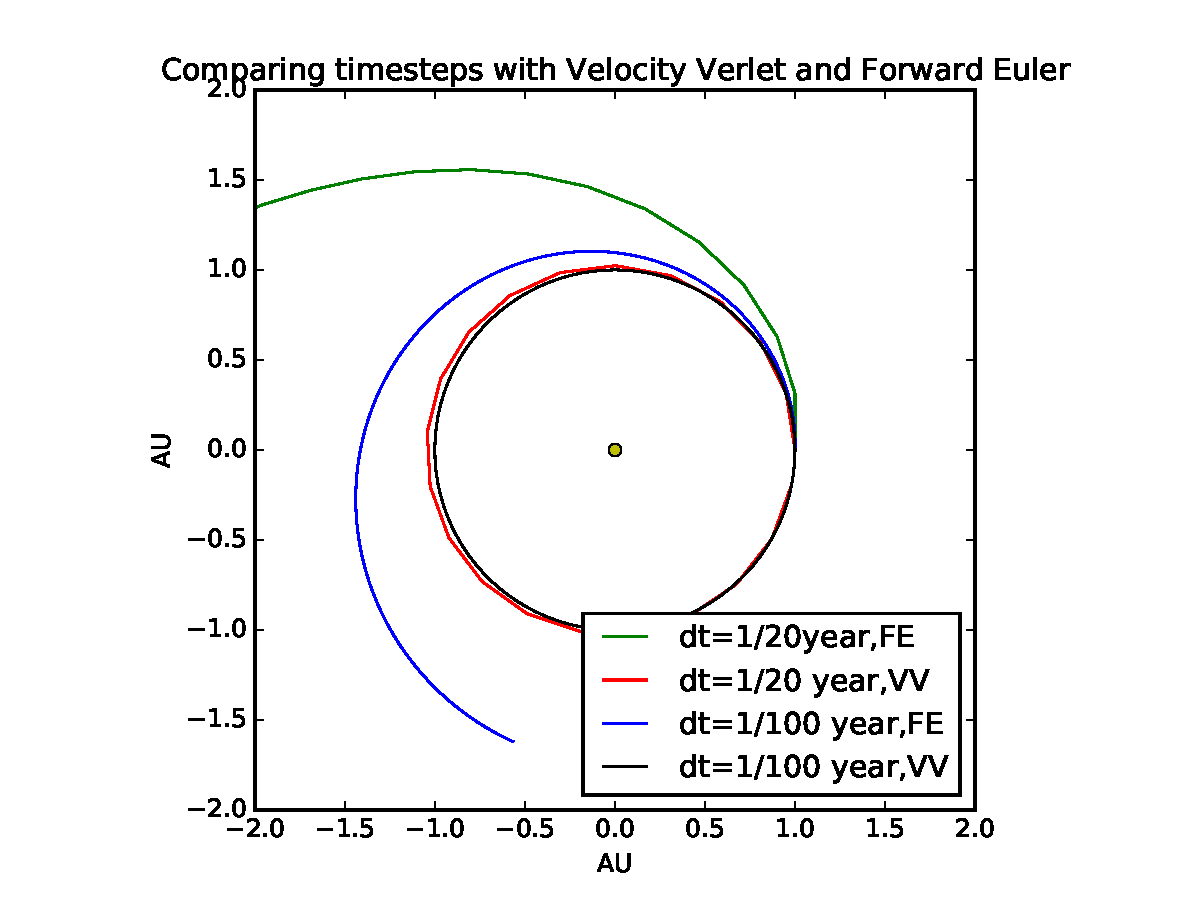
\includegraphics[width=\textwidth]{fig/timestep_test.pdf}
\caption{Comparing Forward Euler and Velocity Verlet with the same time steps for an Earth-Sun system}
\label{fig:timestep_test}
\end{figure}


\subsubsection{Escape Velocity}
The analytical escape velocity at a distance $r$ from an object with mass $M$ is given as $\sqrt{\frac{2GM}{r}}$. Inserting the mass of the sun(1 Solar Mass), and the Earth-Sun distance(1 AU), we arrive at the escape velocity
\begin{equation}
v_{\mathrm{esc}} = \sqrt{\frac{2\cdot 4\pi^2 \cdot 1}{1}} = \sqrt{8}\pi = 2.8284\pi \mathrm{AU}/\mathrm{year} \label{eq:escape_velocity}
\end{equation}

\begin{figure}[ht]
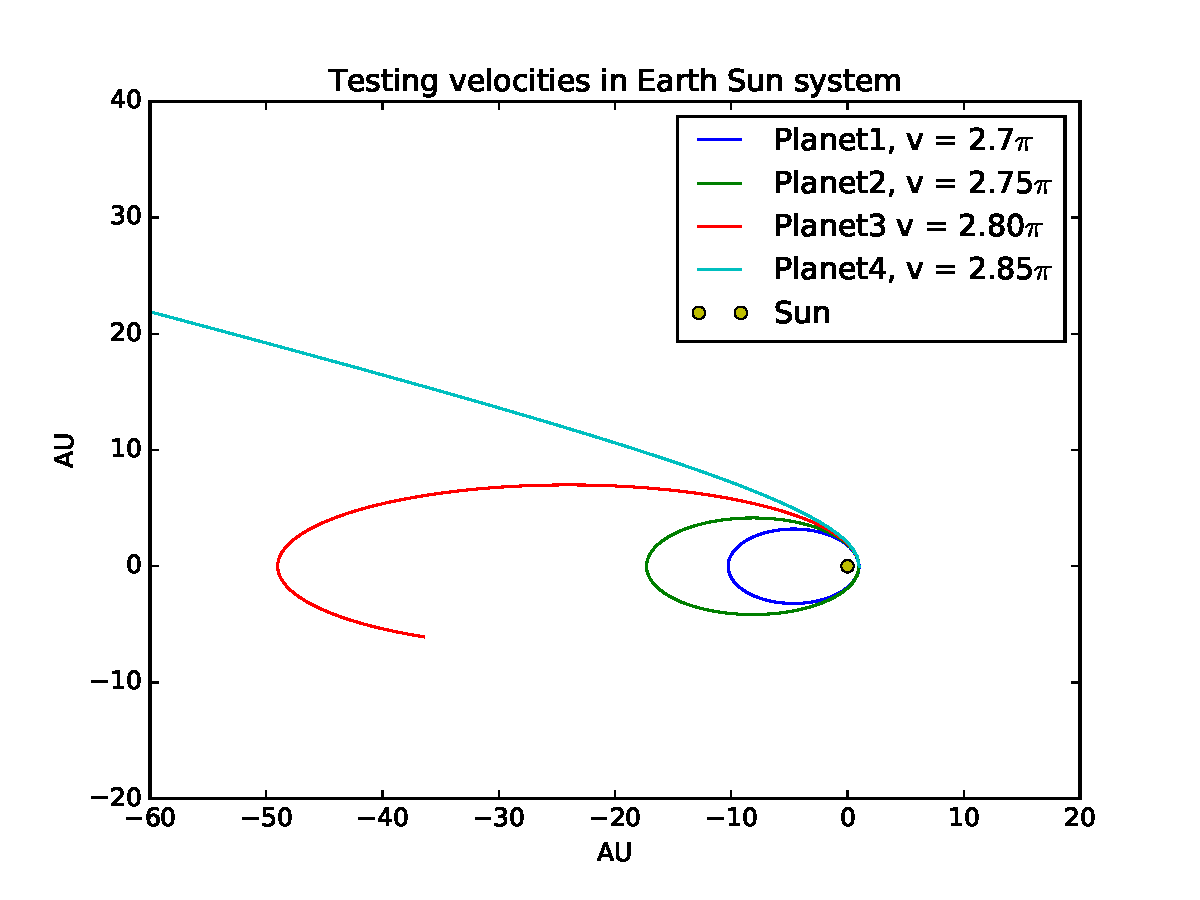
\includegraphics[width=\textwidth]{fig/escape_velocity.pdf}
\caption{Planets 1-3 stay in orbit, while planet 4 escapes the solar system.}
\label{fig:escape_velocity}
\end{figure}

From \vref{fig:escape_velocity}, we see that the escape velocity of the Earth, $v_{\mathrm{esc}} \in (2.8\pi, 2.85\pi)$, which is in alignment with \ref{eq:escape_velocity}


\subsubsection{Conservation of Energy and Angular Momentum}
Because we have an isolated system without external forces, we expect the total mechanical energy and angular momentum of the system to be conserved. In addition, if the planets orbit is circular, we expect the kinetic and potential energy to be respectively conserved. This is because the gravitational force from the sun always stays orthogonal on the planets velocity, meaning no work is done on the planet, and potential and kinetic energy stays unchanged.

\begin{figure}[ht]
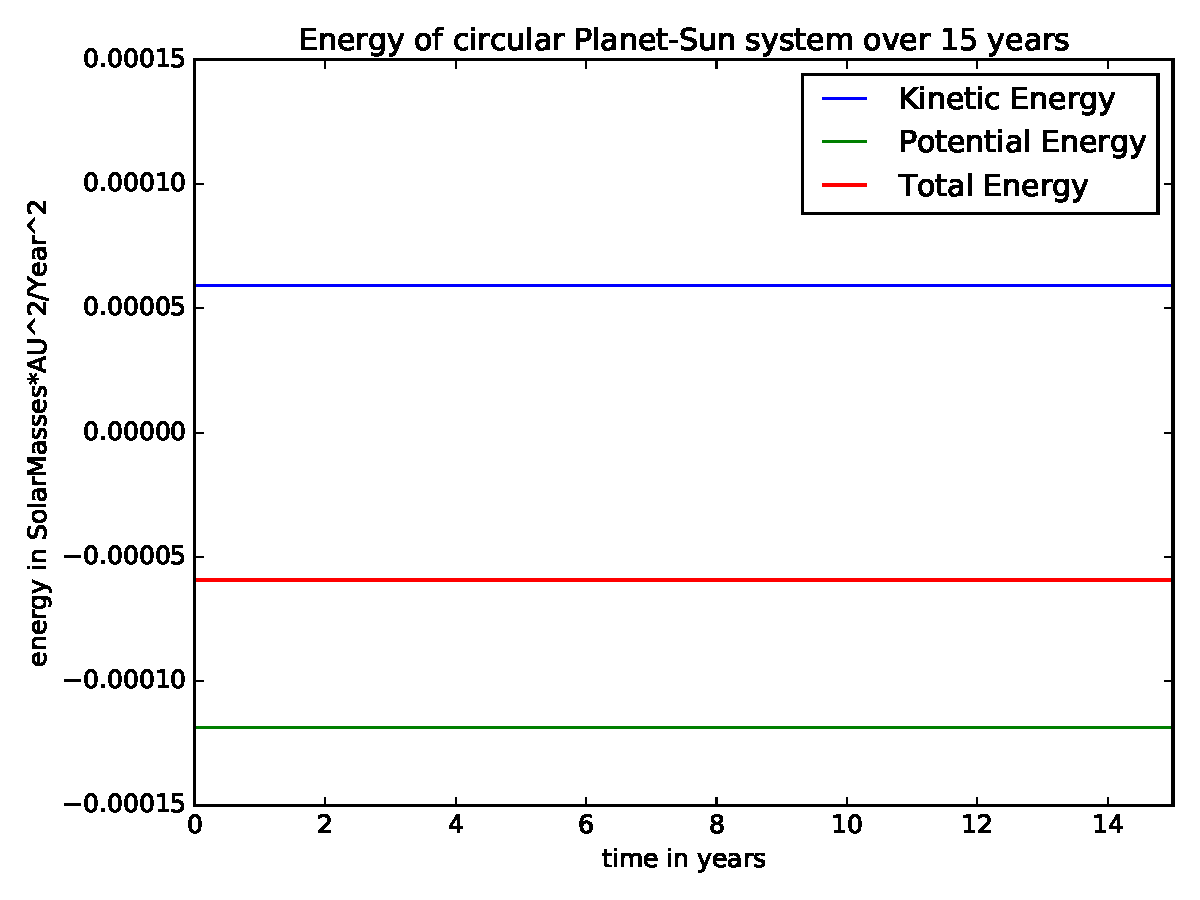
\includegraphics[width=\textwidth]{fig/energy_conservation_v=2pi.pdf}
\caption{Energy conservation with $v = 2\pi$}
\label{fig:energy_conservation_circular}
\end{figure}

\begin{figure}[htb]
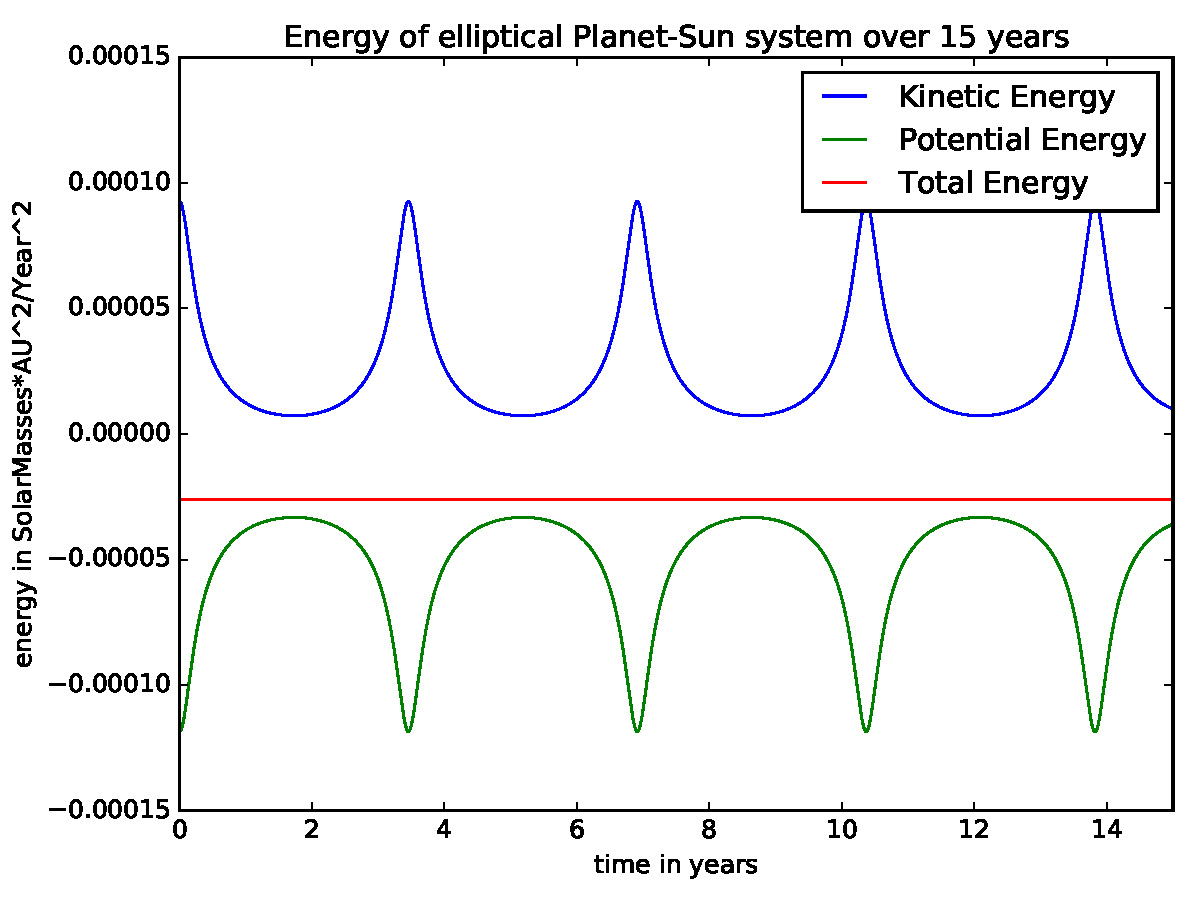
\includegraphics[width=\textwidth]{{fig/energy_conservation_v=2.5pi}.pdf}
\caption{Energy conservation with $v = 2.5\pi$}
\label{fig:energy_conservation_elliptical}
\end{figure}

From \vref{fig:energy_conservation_circular} and \vref{fig:energy_conservation_elliptical}, we see that the energy is indeed conserved.

\begin{lstlisting}[basicstyle=\footnotesize, frame=single, label={lst:preservation},caption=Preservation of center of mass and angular momentum]
Center of mass at beginning of simulation, and after 15 years:
[ 0.  0.]
[ -3.58083178e-18  -8.47472594e-19]
Relative error in angular momentum over 15 years: -6.105258e-14
\end{lstlisting}

From listing \vref{lst:preservation}, we see that the center of mass does remain in the origin (within machine precision). We also note that the relative error in angular momentum is very small.

\subsection{Three-body system}
Throwing Jupiter into the party, we can play around with the masses to see the effect on the orbits.

Note that for these simulations, we disable the automatic adjustment of the Sun, as that depends on the other celestial bodies having masses that are several orders of magnitude smaller.

With Jupiter having 10 times its real mass, we see from \vref{fig:jupiter:10times} that the Earth's orbit is slightly affected, deviating from the circular orbit we would expect.

\begin{figure}[htb]
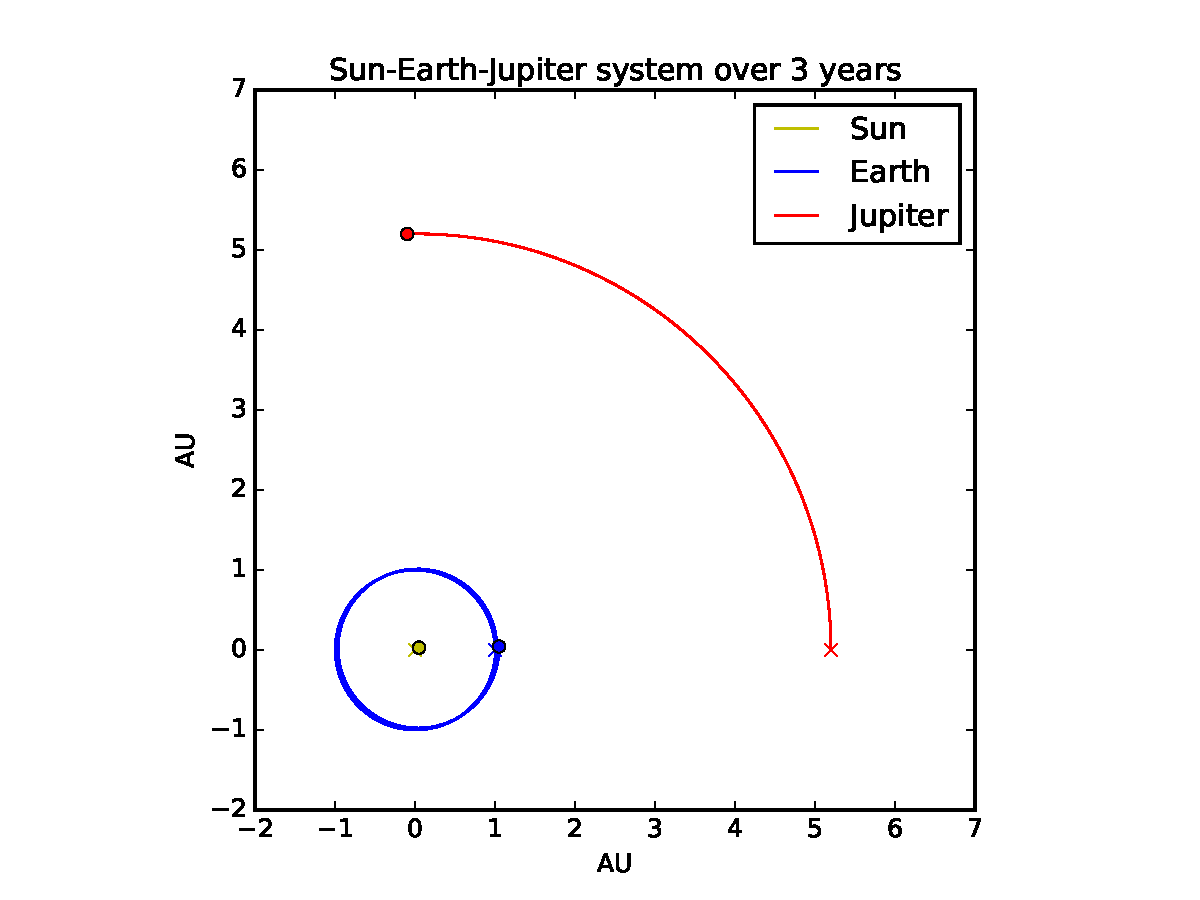
\includegraphics[width=\textwidth]{fig/jupitermass_10.pdf}
\caption{Jupiter with 10 times its real mass}
\label{fig:jupiter:10times}
\end{figure}

\begin{figure}[htb]
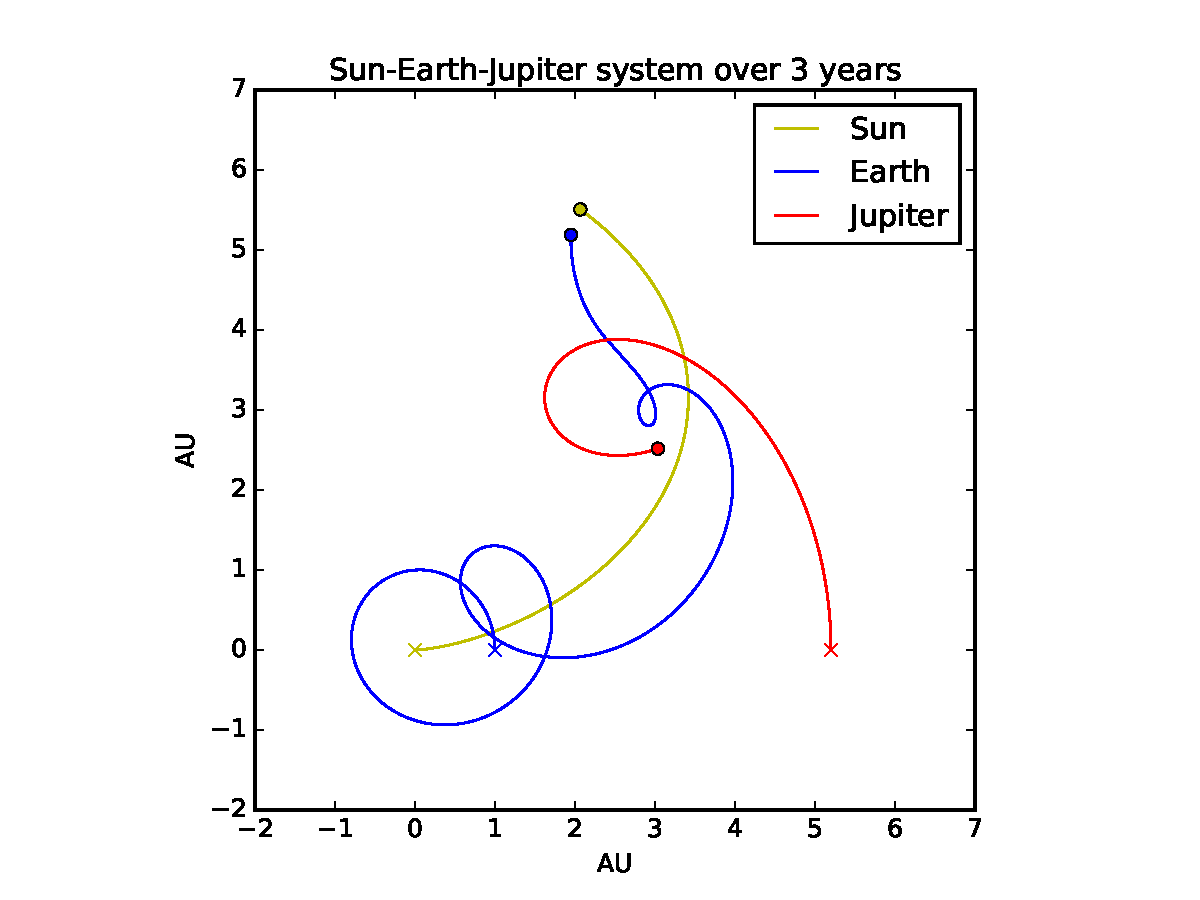
\includegraphics[width=\textwidth]{fig/jupitermass_1000.pdf}
\caption{Jupiter with 1000 times its real mass}
\label{fig:jupiter:1000times}
\end{figure}

\section{Conclusion}\label{sec:conclusion}
We have shown the extreme precision of the Velocity Verlet algorithm in regard to position-dependent forces, far outranking the Forward Euler method.
We then observed that the precession of Mercurys perhelion can only be accurately explained with the introduction of general relativity.
We have observed the large stability of ordinary planitary orbits, and increadible unstability of a planitary system with several massive objects, like our Sun-Jupiter system.

%\bibliographystyle{plain}
%\bibliographystyle{siam}
\bibliographystyle{IEEEtran}
\bibliography{../papers}{}

\end{document}
\grid
\grid
